\chapter{Related Work}

\section{Graph Theory Basics}

In this section some graph theory related notation is defined which is used during this thesis.
A graph is a mathematical construct that can be used to model and explore the relationship between objects. 
More formally, a graph \cite{Thulasiraman1992} is a ordered pair of finite sets \(G = (V, E)\), whereas \(V\) denotes the set of \emph{vertices} (i.e., the objects) and \(E \subseteq [V]^2 \) the set of \emph{edges} (i.e., the relationships between the objects).
It is common to write \(V(G)\) and \(E(G)\) to refer to the set of vertices, respectively the set of edges, that are associated with a graph \(G\).
An edge \(\{v_1, v_2\} \in E(G)\) is an unordered pair of two vertices.
This means that there is not distinction between the two edges \(\{v_1, v_2 \}\) and \(\{v_2, v_1\}\). 
A graph with this property is called a \emph{undirected} graph.
However, it is also possible to define edges as ordered pairs, so that each edge does have a start- and endpoint. 
Such a graph is called a \emph{directed} graph.
An edge of the form \(\{v_i, v_i\} \in E(G)\) is called a \emph{self-loop} of the vertex \(v_i\).
Furthermore, it is possible that two distinct vertices are joined by multiple edges. 
Such edges are referred to as \emph{parallel} edges.
A graph that has no parallel edges and no self-loops is denoted as a \emph{simple} graph.
Figure \ref{fig:example_graphs} depicts two examples for graphs.


\begin{figure}
   \centering
   \begin{subfigure}[t]{0.45\textwidth}
     \centering
     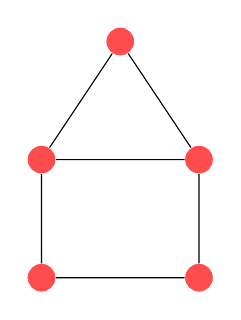
\begin{tikzpicture}[node/.style={circle,fill=red!70,minimum size=1em,inner sep=3pt]}]
       \node[node] (1) at (0, 0) {};
       \node[node] (2) at (-1, -1.5)  {};
       \node[node] (3) at (1, -1.5) {};
       \node[node] (4) at (-1, -3) {};
       \node[node] (5) at (1, -3) {};
       
       \draw (1) -- (3);
       \draw (1) -- (2) -- (4) -- (5) -- (3) -- (2);
     \end{tikzpicture}
     \caption{A undirected simple graph.}   
   \end{subfigure}
   ~
   \begin{subfigure}[t]{0.45\textwidth}
     \centering
     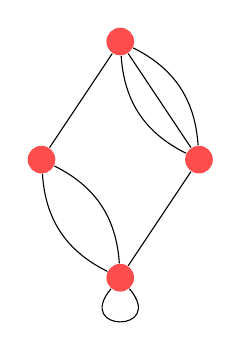
\begin{tikzpicture}[every loop/.style={}, node/.style={circle,fill=red!70,minimum size=1em,inner sep=3pt]}]
       \node[node] (1) at (0, 0) {};
       \node[node] (2) at (-1, -1.5)  {};
       \node[node] (3) at (1, -1.5) {};
       \node[node] (4) at (0, -3) {};
      
       \draw (1) -- (2);
       \draw (1) -- (3) -- (4);
       \path (2) edge [bend left] (4);
       \path (2) edge [bend right] (4);
       \path (3) edge [bend left] (1);
       \path (3) edge [bend right] (1);
       \draw (4) edge [in=-50,out=-130,loop] (4);
     \end{tikzpicture}
     \caption{A undirected graph with a self-loop and parallel edges.}
   \end{subfigure}
   
   \caption{Graphical representation of two graphs with different properties.} 
   \label{fig:example_graphs}
\end{figure}

The \emph{order} of a graph is the number of vertices (i.e., the cardinality of the vertex set) and is denoted as \(n = |V|\). 